\documentclass{standalone}
\usepackage{tikz}
\begin{document}
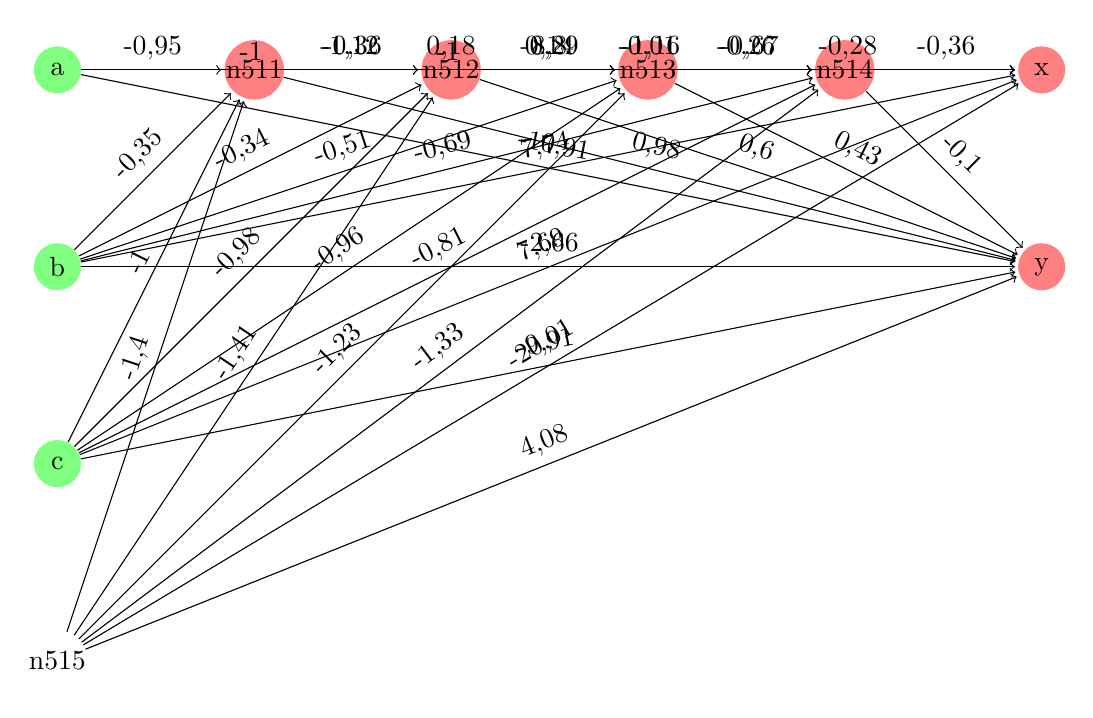
\begin{tikzpicture}[shorten >=1pt,->,draw=black!,node distance=2.5cm]
\tikzstyle{neuron}=[circle,fill=black!25,minimum size=17pt,inner sep=0pt]
\tikzstyle{constant}=[neuron, fill=white!50];
\tikzstyle{identity}=[neuron, fill=green!50];
\tikzstyle{sigmoid}=[neuron, fill=red!50];
\node [identity] (a) {a};
\node [identity,below of=a] (b) {b};
\node [identity,below of=b] (c) {c};
\node [constant,below of=c] (n515) {n515};
\node [sigmoid,right of=a] (n511) {n511};
\node [sigmoid,right of=n511] (n512) {n512};
\node [sigmoid,right of=n512] (n513) {n513};
\node [sigmoid,right of=n513] (n514) {n514};
\node [sigmoid,right of=n514] (x) {x};
\node [sigmoid,below of=x] (y) {y};
\path[every node/.style={sloped,anchor=south,auto=false}]
(b) edge node {-2,66} (y)
(b) edge node {7,74} (x)
(b) edge node {-0,34} (n512)
(b) edge node {-0,35} (n511)
(b) edge node {-0,69} (n514)
(b) edge node {-0,51} (n513)
(a) edge node {8,8} (x)
(a) edge node {-1} (n514)
(a) edge node {-0,95} (n511)
(a) edge node {-10,91} (y)
(a) edge node {-1,12} (n513)
(a) edge node {-1} (n512)
(n512) edge node {0,6} (y)
(n512) edge node {-0,67} (x)
(n512) edge node {-0,01} (n514)
(n512) edge node {0,14} (n513)
(c) edge node {7,69} (x)
(c) edge node {-1} (n511)
(c) edge node {-9,91} (y)
(c) edge node {-0,96} (n513)
(c) edge node {-0,98} (n512)
(c) edge node {-0,81} (n514)
(n511) edge node {-1,16} (x)
(n511) edge node {0,98} (y)
(n511) edge node {0,18} (n513)
(n511) edge node {-0,36} (n512)
(n511) edge node {-0,29} (n514)
(n514) edge node {-0,1} (y)
(n514) edge node {-0,36} (x)
(n513) edge node {-0,28} (x)
(n513) edge node {0,43} (y)
(n513) edge node {-0,26} (n514)
(n515) edge node {4,08} (y)
(n515) edge node {-1,4} (n511)
(n515) edge node {-20,01} (x)
(n515) edge node {-1,33} (n514)
(n515) edge node {-1,41} (n512)
(n515) edge node {-1,23} (n513)
;\end{tikzpicture}
\end{document}